\chapter{Delay}
\graphicspath{{foto/Chap2/}}
\label{sec:Delay}
\section{Delay computation}
Each operation on the memory requires a certain time to be performed. In the model used four operations have been defined: precharge, read, write and erase. The only delays that have been considered in the model are precharge and read ones, because they are the only ones that can be evaluated in a qualitative way by using the parameters defined previously. The write and erase delays depend on physical and technological parameters of the transistors that are involved in the tunnel effect, so they are hard to model. Another thing that has been considered is the fact that the most common operation on a NAND memory is the read operation (with its precharge). So, we estimate the delay due to a precharge and subsequent read operation, taking into account not only the memory array, but also all the hardware components around it, from the decoding of the address bits to the switching of the sense amplifier and the selection of the column bit to be read.

\subsection{Precharge unit delay}
The precharge unit is driven by an \textit{Enable} signal coming from a control unit internal to the memory (which we won't consider in this analysis). The precharge unit is simply a pmos transistor, connected from one side to the supply voltage and from the other side to the bitline. The \textit{Enable} signal has to discharge the gate capacitance of this pmos, in order to make it able to switch, so the delay associated to this operation is:
$$\tau=R_{ext,pu,driver}(C_{ext,pu,driver}+C_{g,pre})$$

After the switching of the precharge unit, the bitline takes a certain time to be charged. This delay is:
$$\tau=\frac{(C_{bl,wire} \cdot L_{bl})V_{bl,prec}}{I_{on,driver}}$$
where L is the length of the array of memory.

\subsection{Block decoder delay}
To model the delay of this and of the other similar components we used the classical model used to determine the delay of a logic gate. The dynamic NAND decoder, in fact, is built by a precharge pmos followed by a stack of nmos transistors, as in the following picture:

\begin{center}
	\begin{figure}[H]
		\centering
		\includegraphics[scale = 0.6]{NANDdec.png}
		\caption{Core of the dynamic NAND decoder}
	\end{figure}
\end{center}

Only one among these stacks of transistors will switch, making the corresponding output to go low, and so the whole structure behaves just like an ordinary logic gate.

In addition to this structure, of course, we have also the inverters placed on the input, to get also the complemented version of the address bits. Moreover, we also have a set of inverters on the output lines: the active output of a NAND decoder, in fact, is low; the output lines of the block decoder instead, as can be observed from the full scheme of the memory reported below for convenience, are needed to switch one of the nmos transistors which connect the output from the row decoder to the wordlines, and of course the nmos transistors are turned on by a high voltage. 

\begin{center}
	\begin{figure}[H]
		\centering
		\includegraphics[scale=0.6]{3dmemory-SLICE_SCHEME.pdf}
		\caption{Full scheme of the memory}
	\end{figure}
\end{center}

We consider the address bits in input to the block decoder, including their complemented version, to be stable from the beginning, while we have to take into account the delay contribution due to the inverters on the output lines. 

As mentioned before, we model this delay contribution like the delay of a traditional logic gate, so:
$$\tau_{block,dec}=R_n(C_d+C_L)$$
$R_n=Stack_n\cdot R_{eq,sdec,n}$ is the equivalent output resistance due to the stack of the nmos transistors, where $R_{eq,sdec,n}$ is the output resistance of a single nmos transistor and $Stack_n=Block_Address$ is the number of nmos transistors forming the stack. $C_d=C_{d,sdec,pcharge}+C_{d,sdec,eval}$ is the self-load capacitance due to the drain-bulk capacitance of the pmos and of the nmos on the output line. $C_L=C_{g,sdec,inv,p}+C_{g,sdec,inv,n}$ finally is the load capacitance due to the presence of the inverter on the output line. \\

\subsubsection{Output inverter}
The delay of the inverter on the output line is computed following the same model: 
$$\tau_{block,inv}=R_p(C_d+C_L)$$
$R_p=1\cdot R_{eq,sdec,inv,p}$ is the output resistance of the inverter; here we have focused on the pmos because we are interested in the case in which its output is driven high, since that is the only case in which it is able to switch the pass transistor it has as a load. $C_d=C_{d,sdec,inv,p}+C_{d,sdec,inv,n}$ as usual is the self-load capacitance of the gate. $C_L=C_{g,rowpass}(N_{wl}+2)+C_{g,slice}$ is the full load of each inverter on the output of the block decoder. This inverter in fact has to drive the $N_{wl}$ pass transistors connected to the wordlines, plus one SST and one GST (hence the $+2$), plus the pass transistor which allows the read bit to go out from the block (hence the $+C_{g,slice}$).

\subsection{Row decoder}
The next contribution is the one due to the row decoder. The block decoder and the row decoder work together, but if the number of address bits in input to the row decoder is much larger than the ones in input to the block decoder (and this is likely), also the stack of the nmos transistor will be larger and the row decoder will result to be slower than the block decoder. However, the block decoder has a load capacitance considerably higher than the one of the row decoder: not only it drives more transistors, but the capacitance to be considered in its case is the gate capacitance, which is much larger than the drain capacitance of the same transistor. So, since we don't know, at least using parametric values, which delay will be larger, we decided to compute both and to consider at the end, in the final value of the delay, only the largest one. The difference, as said, may be either in the contribution due to the decoder structure or in the contribution due to the driving capabilities of the inverter on the output line: for example, the block decoder may have a lower number of stack transistor, but the load of its inverter may be much larger. So, in the end, we must compare separately $\tau_{block,dec}$ with $\tau_{row,dec}$ and $\tau_{block,inv}$ with $\tau_{row,inv}$. The critical path delay will be determined by the largest from each couple of comparisons. We sum up below the structural details interested in this analysis for sake of clarity.

\begin{center}
	\begin{figure}[H]
		\centering
		\includegraphics[scale=0.6]{blockrowdec.png}
		\caption{Row decoder and block decoder timing}
	\end{figure}
\end{center}

Since the structure of the decoder is the same, also the model to compute its delay doesn't change:
$$\tau_{row,dec}=R_n(C_d+C_L)$$
$R_n=Stack_n\cdot R_{eq,rdec,n}$ is the equivalent resistance due to the stack of the nmos transistors, and $Stack_n=Row_Address$. $C_d=C_{d,rdec,pcharge}+C_{d,rdec,eval}$ is the self-load capacitance. $C_L=C_{g,rdec,inv,p}+C_{g,rdec,inv,n}$ is again the load capacitance due to the inverter on the output.

\subsubsection{Word line delay}
The inverter on the output of the row decoder is taken into account in this section, since it works as driver for the charge of the selected word line. Due to the presence of the pass transistor between the row decoder and the word line, which represents the load to be charged, this time we have to use the Elmore model to represent the situation.

\begin{center}
	\begin{figure}[H]
		\centering
		\includegraphics[scale=0.6]{wordlinedelay.png}
		\caption{Elmore model for the wordline delay}
	\end{figure}
\end{center}

The equation to compute the delay with the Elmore model becomes:
$$\tau_{row,inv}=R_{eq,inv}(C_{d,inv}+C_{d,pass}+C_L)+R_{eq,pass}(C_{d,pass}+C_L)$$
$R_{eq,inv}=R_{eq,rdec,inv,p}$ is the equivalent resistance from the output of the inverter (again, we focus on the pmos because the interesting case is when its output goes high). $C_{d,inv}=C_{d,rdec,inv,p}+C_{d,rdec,inv,n}$ is the self-load capacitance of the inverter. $R_{eq,pass}=R_{eq,rowpass}$ and $C_{d,pass}=C_{d,rowpass}$ are respectively the equivalent resistance and drain capacitance of the pass transistor which drives the wordline. Here we consider only the inverters driving the transistors GST (ground select transistor) and SST (string select transistor). Actually all the other lines coming out from the decoder are connected to different transistors, the floating gate transistors constituting the memory cells. Since the capacitance of a floating gate transistor is smaller than the one of a traditional transistor, the worst case is given for $C_L=C_{g,pt}N_{bl}$, where $C_{g,fg}$ is the gate capacitance of a GST or SST, and $N_{bl}$ is the number of GST or SST per each wordline. 



\subsection{Bit line delay}
During the read operation, all the strings in the slice are connected to the bit line. Depending on the value memorized in the cell, they can discharge the bit line capacitance or act as an open circuit. The variation of the bitline capacitance provides the value of the cell which is measured through external components (sense amplifiers). The duration of the evaluation phase of the charge is the same for both 1s and 0s. It is timed accordingly with the delay in the discharge phase because, if the string act as an open circuit, the capacitance of the bit line remains the same, so there is no delay. The strings are read in parallel, hence the delay is the one corresponding to a single pillar. 

An Elmore model has been used for the string where each FGT and SST/GST is modelled with a capacitance and a resistance as shown in the picture below.

So, in this phase, the delay has been evaluated by using the following formula:
$$\tau_{eval}=C_1 \cdot R_1 + C_2 \cdot (R_1+R_2) + C_3 \cdot (R_1+R_2+R_3)+...$$

\begin{figure}[h] 
	\begin{center}
		\includegraphics[width=.3\textwidth]{Elmore_model}
	\end{center}
	\caption{Elmore model for the bitline delay} 
\end{figure}
 
We assume, however, that only a small part of this delay will be really needed in the estimation of the total delay, since we have a sense amplifier connected at the end of each bitline. The sense amplifier is at the beginning in a metastable state, but as soon as it senses a voltage difference between its input (the bitline) and the reference value provided from the external, it switches to a stable state, forcing at the same time a fast charge/discharge of the input line itself. So, the formula actually used in our computations includes also a generic $K_{SA}$ factor (which may be 5\%, for example):
$$\tau_{eval}=K_{SA}(C_1 \cdot R_1 + C_2 \cdot (R_1+R_2) + C_3 \cdot (R_1+R_2+R_3)+...)$$

\subsection{Sense amplifier delay}
The sense amplifier is made with two cross coupled inverters that are brought to a metastable state and then are applied a voltage difference by means of the input bitline. Note that in this amplifier, input and output are somehow corresponding. The schematic of the component is shown below:

\begin{figure}[h] 
	\begin{center}
		\includegraphics[scale=0.4]{senseamplifier.png}
	\end{center}
	\caption{Sense amplifier structure} 
\end{figure}

Its delay is described by a simple RC model:
$$\tau=R_{eq,sa,mod,parallel}(C_{d,sa,p}+C_{d,sa,n}+C_{g,sa,p}+C_{g,sa,n}+(C_{bl,wire}\cdot L_{bl})+C_{d,colpass})$$
In this equation we take into account the equivalent resistance of the sense amplifier, which drives its self-load capacitance, the capacitance due to the gate of the cross-coupled inverter, the capacitance of the bitline, plus the drain capacitance of the pass transistor connected at the bottom of the bitline and whose gate terminal is driven by the column decoder.

\subsection{Delay of the column pass transistor and of the slice transistor}
Finally, the last contribution to the delay is given by the two pass transistors we have before the output from the block. The former is driven by the column decoder (by the inverter on its output), the latter by the block decoder (by the inverter on its output). We don't consider the delay of the column decoder, because it works together with the block decoder and the row decoder, and even if its delay was longer than the largest between the other two, we have also all the contributions from the charging of the wordline and from the discharging of the bitline and the switching of the sense amplifier, so at this point the output of the column decoder will have for sure become stable.   

To compute the delay due to the two pass transistors we use again the Elmore model:
$$\tau=R_{eq,pass}(C_{d,pass}+C_{d,slice}+C_L)+R_{eq,slice}(C_{d,slice}+C_L)$$

\begin{figure}[h] 
	\begin{center}
		\includegraphics[scale=0.6]{columnpassdelay.png}
	\end{center}
	\caption{Elmore model for the pass transistors delay} 
\end{figure}

$R_{eq,pass}=R_{eq,colpass}$ is the equivalent resistance of the pass transistor driven by the column decoder, whereas $C_{d,pass}=C_{d,colpass}$ is its self-load capacitance. $R_{eq,slice}$ and $C_{d,slice}$ are the analogous parameters for the pass transistor driven by the inverter out from the block decoder. $C_L$ is unknown and in our analysis is assumed to be an open circuit. \\

\subsection{Total delay}
The total delay is computed as the sum of all the contributions described up to now (with the exception of the block decoder and the row decoder, as already described), multiplied by 0.69.

\section{Simulation result}
To verify the plausibility of our computations we assigned a reasonable value to each of the parameters involved in the equations. We also made the number of wordlines and bitlines change in a well defined range, to analyse how the delay changes if we vary the dimensions of the memory array. In particular, the array of values we considered for both $N_{wl}$ and $N_{bl}$ is $[64, 128, 256, 512, 1024, 2048]$. For each simulation point we assumed that $N_{bl}=N_{wl}$, because usually the memory arrays are made as square as possible, for reasons of space availability on the board.\\

The result we obtained is reported in the figure below. 

\begin{figure}[h] 
	\begin{center}
		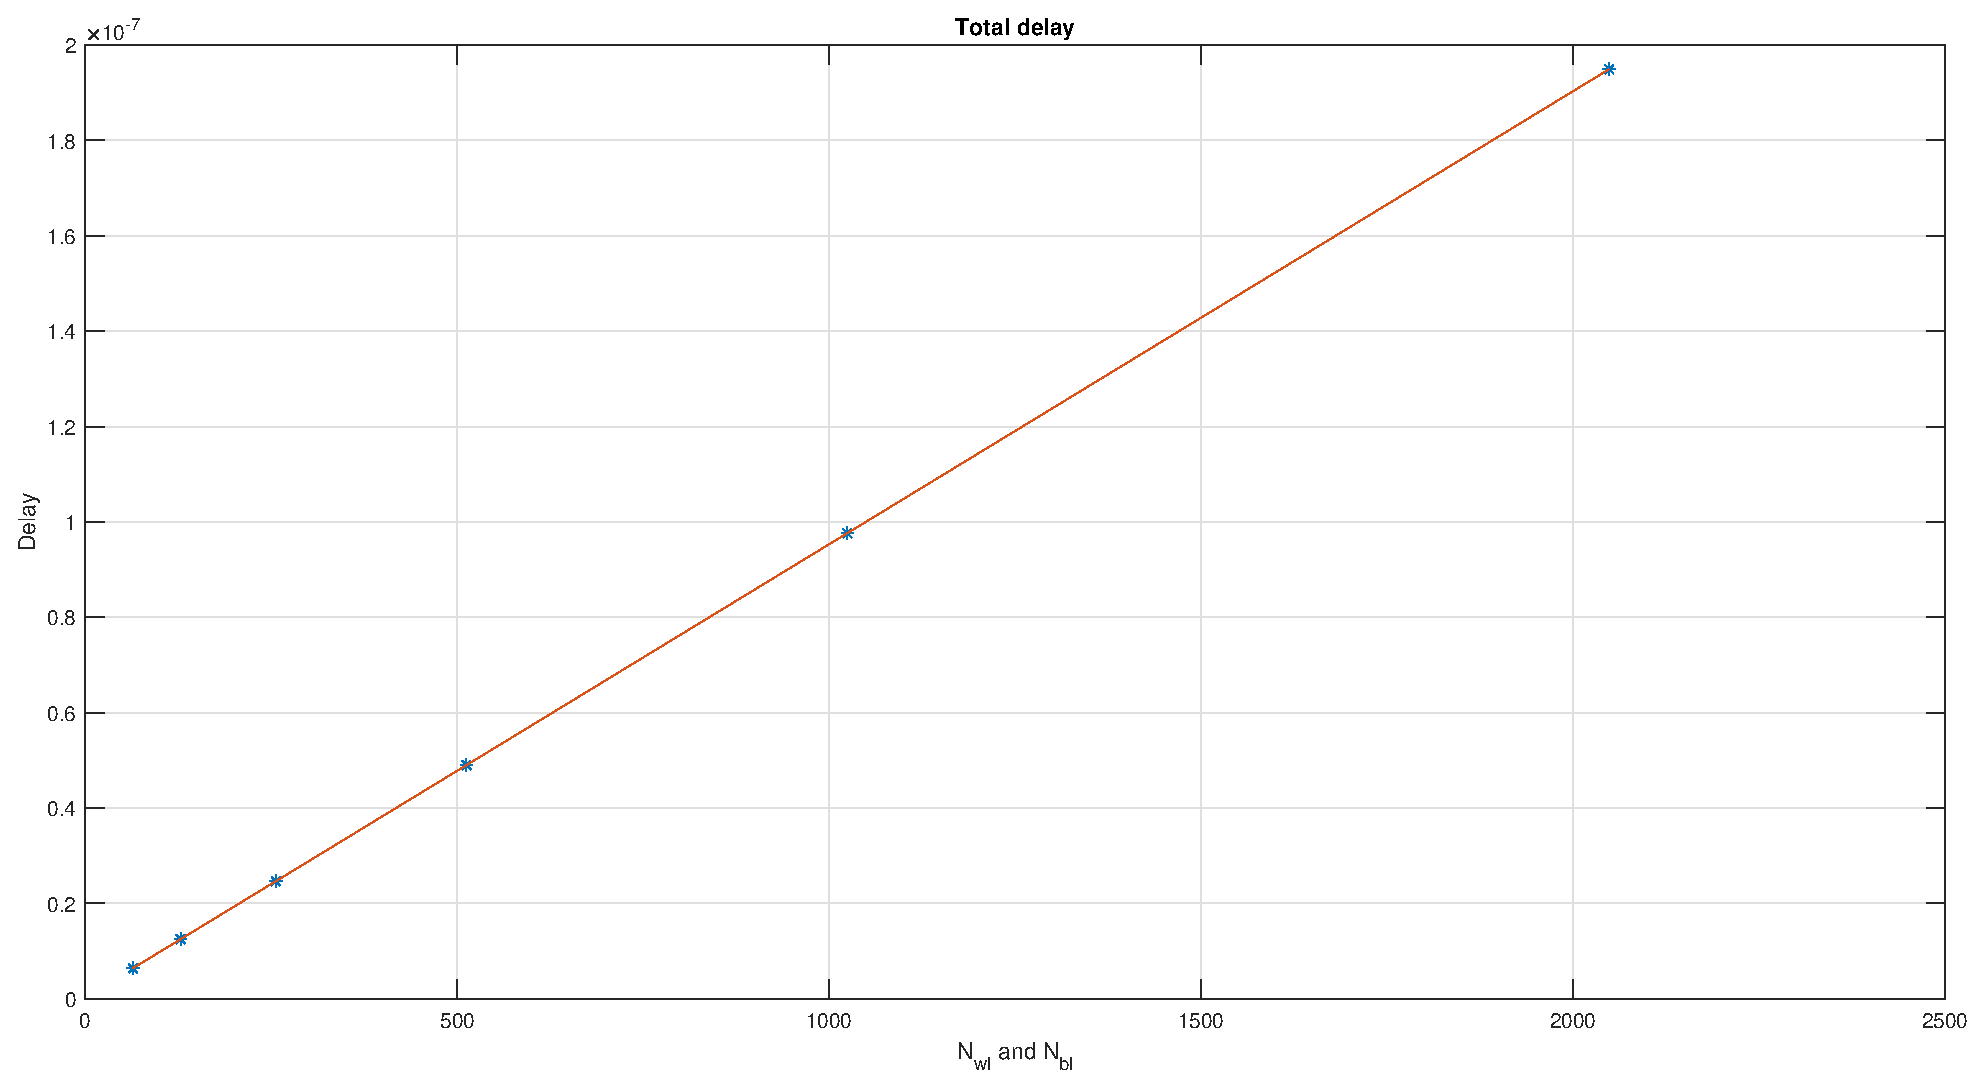
\includegraphics[scale=0.4]{delay_sim.eps}
	\end{center}
	\caption{Simulation of the delay varying the size of the memory array} 
\end{figure}

The behaviour represented is reasonable: in all the contributions previously discussed we always have at most a linear dependence on $N_{wl}$ or $N_{bl}$; some terms are independent from the variations of these two parameters and they partially contribute to the offset that can be observed on the 64x64 simulation point. Instead, we never have a square dependence on either of the two parameters, so an overall linear behaviour is perfectly reasonable.\\

So, with the values chosen for the parameters involved, the total delay of a precharge\&read operation spans between 6.43ns, in the 64x64 case, and 195ns in the 2048x2048 case.